\subsection{Prerequisites}\label{sec:33prereq}
\subsubsection{Cross-section data input}\label{sec:xsect}
%The ionisation cross-section $\Sigma_{ION}$ for Hydrogen ions as a function of~$T_i$
Cross-section data will be obtained from the ADAS library~\cite{adaswebsite}.
Cross-section data $\langle\sigma v\rangle$ averaged over a Maxwellian velocity distribution suitable for
use by a fluid model of the plasma edge is shown in \Fig{xsects}, from Havlickova~et~al.~\cite{Ha13Benc}.
The dominant relevant reactions affecting both neutrals and plasma in the graph are
\begin{eqnarray}
\mbox{Ionisation (ION)} \;\;\; e^-+ H &\rightarrow& H^+ + e^-+ e^-\\
\mbox{Charge-exchange (EXC)} \;\;\; H + H^+ &\rightarrow& H^+ + H
\end{eqnarray}
\begin{figure}
\centerline{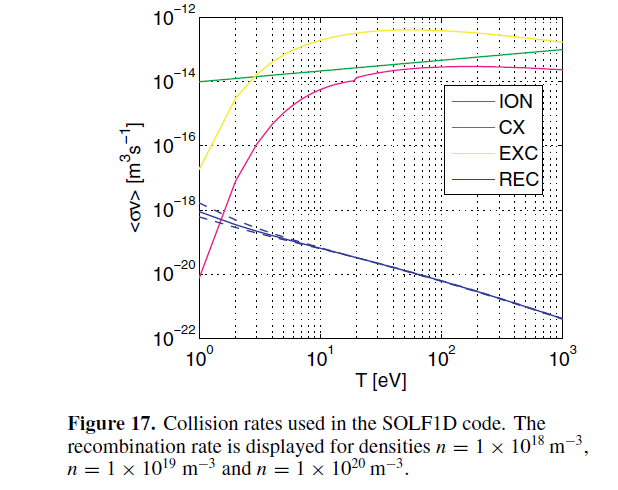
\includegraphics[width=10cm]{../png/Ha13Benc_xsects.png}}
\caption{Extract from publication indicated in the text.  \label{fig:xsects}}
\end{figure}

\subsection{Physical Models}\label{sec:models}
\subsubsection{Introductory model}\label{sec:intromodel}
Perhaps the simplest model to consider is that for ionisation of neutrals by electron impact.
A simple model for ionisation can be written as:
\begin{eqnarray}
\frac{\partial f_{n}}{\partial t} & = & \ldots-R_{ION}n_{i}f_{n}\\
\frac{\partial n_{i}}{\partial t} & = & \ldots+R_{ION}n_{i}n_{n}
\end{eqnarray}
where $R_{ION}$ ($\langle\sigma v\rangle_{ION}$ elsewhere) is a constant ionisation rate, $f_{n}$
is the distribution function for the neutrals, $n_{i}$ and $n_{n}$
are the ion and neutral densities. The quasineutrality assumption implies
$n_{e}=n_{i}$. So the `source term' in the plasma density equation is
\begin{equation}
S_{ION}({\bf x})\equiv R_{ION}n_{i}n_{n}=R_{ION}n_{i}\int d^{3}v\,f_{n}(\boldsymbol{v})
\end{equation}
the integral in which converts, for number densities, into weighted counts of the number
of particles within a given spatial volume about point~${\bf x}$.

\begin{figure}
\centerline{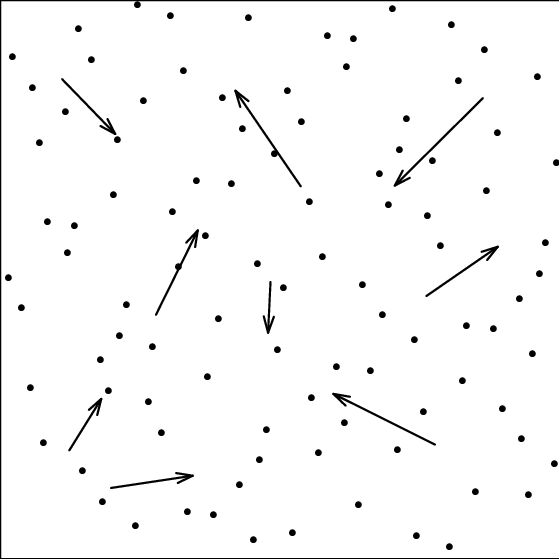
\includegraphics[width=6cm]{../png/harrows.png}}
\caption{Configuration for ionisation.
Neutrals, indicated by arrows, moving against a background of thermal electrons shown
as dots.  \label{fig:harrows}}
\end{figure}
The loss term in the neutral density equation is computed using Monte Carlo
techniques, cf. Verboncouer~\cite{Ve05Part}, configuration sketched in \Fig{harrows}. The probability of ionisation of a
particle at time~$t_n$ travelling with velocity~${\bf v}_p$ in the following
interval of~$\Delta t$ is
\begin{equation}
\mathrm{p}_p(t_n) = 1-\exp\left(-n_e \sigma_{ION} |{\bf v}_p| \Delta t\right)
\end{equation}
where the cross-section for ionisation is $\sigma_{ION}$. Provided the background
density~$n_e$ is approximately constant in space and time, and $\sigma_{ION}$
variation with energy~$\mathcal{E}$ is assumed to be  negligible, taking 
for example
\begin{equation}
\nu_{\sigma max}= \max_{\bf x} \{n_t({\bf x})\}\max_{\mathcal{E}}\{\sigma_T(\mathcal{E}) |{\bf v}|\}
\end{equation}
then for every particle, provided all particles have the same weight (ie.\ identical
superparticles), approximately
\begin{equation}
\mathrm{p}_p =\mathrm{p}_T= 1-\exp\left(-\nu_{\sigma max} t\right)
\end{equation}
and the number of neutrals that undergo ionisation in volume~$\Delta V$
is $\mathrm{p}_T n_n \Delta V$. Such particles should be chosen at random from those
in ~$\Delta V$.

The Monte Carlo algorithm for selecting which neutrals turn into ions, is simple
provided that particles are distributed at random throughout~$\Delta V$, viz.\ to
obtain a random number~$\xi$ from the uniform distribution on the unit interval
(ie.\ $0<\xi<1$) for each particle in turn and if at the $q^{th}$
$\xi<\mathrm{p}_T$ then  the $q^{th}$~particle  is regarded as ionised at time~$t_n$.
If particles are each allowed a weight~$w_p(t)$  which varies with time, then the 
weight of the neutral may simply be reduced to account for the ionisation
\begin{equation}
w_p(t_n+\Delta t)=\mathrm{p}_p(t_n) w_p(t_n)
\end{equation}

\subsubsection{Detailed model}\label{sec:modet}
For sources in the fluid equations due to ionisation of neutrals by electrons, the
formulae, cf. \Eqr{Snn}{SEn} (\cite[Eqs.(34)-(36)]{Ha13Benc}) are
\begin{eqnarray}
\label{eq:Sne} S^n_e&=& N_n N \langle\sigma v\rangle_{ION} \\
\label{eq:Svn} {\bf S}^{\bf v}_n&=&N_n N \langle\sigma v\rangle_{ION} {\bf v}_n \\
\label{eq:Spe} S^p_e&=& -\frac{2}{3} N_n N \langle\sigma v\rangle_{ION} k I_H\\
\label{eq:Spi} S^p_i&=& \frac{2}{3} N_n N \langle\sigma v\rangle_{ION} (\frac{3}{2} kT_n + \frac{1}{2} m_n {\bf v}_n^2 )
\end{eqnarray}

Note that other effects due to charge-exchange and recombination may be deduced from
the equations in \Sec{sources}. Monte Carlo calculation may then proceed using a total
cross-section for all three interactions.
\subsubsection{Simplified model}\label{sec:modsimp}
For an exploratory calculation with the Hermes-3 equations, the ionisation potential term is an unwelcome complication
and the momentum term is assumed not to contribute to the evolution of the vorticity~$\omega$.
Hence \Eqr{Sne}{Spi} above become
\begin{eqnarray}
\label{eq:Snesimp} S^n_e&=& N_n N \langle\sigma v\rangle_{ION} \\
\label{eq:Svnsimp} {\bf S}^{\bf v}_n&=& {\bf 0} \\
\label{eq:Spesimp} S^p_e&=& 0 \\
\label{eq:Spisimp} S^p_i&=& \frac{2}{3} N_n N \langle\sigma v\rangle_{ION} (\frac{3}{2} kT_n + \frac{1}{2} m_n {\bf v}_n^2 )
\end{eqnarray}
Compared to the introductory model in \Sec{intromodel}, spatial variations in
background density and cross-section are handled by the null collision method, see \Sec{33nasimp}.

Introducing the (super-)particles newly ionised in time interval~$\Delta t$, occupying
positions~${\bf x}_p$ with label~$p$ and weight~$w_p$ and interaction~$I$:
\begin{eqnarray}\label{eq:Spartion}
S^{n}_e V^e \Delta t & \approx & \Sigma_{pI} w_p\delta_D({\bf x}-{\bf x}_p) \\
S^{p}_i V^e \Delta t & \approx &\frac{2}{3} m_n \Sigma_{pI} w_p\delta_D({\bf x}-{\bf x}_p) \frac{1}{2} \mathbf{v}_{n,pI}^2
\end{eqnarray}
where the contribution to the energy in a finite element~$e$ is a sum over all particle
interactions~$I$ that have occurred in~$e$. These values are projected
on the finite element basis as for charge assignments
($\delta_D$ is the Dirac delta function) so that they give rise to source terms
\begin{eqnarray}\label{eq:Sfluidion}
S^{n}_e({\bf x}) V^e \Delta t & = & \Sigma_{e,p} w_p\phi_{e,\xi}({\bf x}_p) \phi_{e,\xi}({\bf x}) \\
S^{p}_i({\bf x})  V^e \Delta t & \approx &\frac{1}{3} m_n \Sigma_{e,p} w_p
\mathbf{v}_{n,p}^2 \phi_{e,\xi}({\bf x}_p) \phi_{e,\xi}({\bf x})
\end{eqnarray}
where $\phi_{e,\xi}$ is the expansion basis as a function of global
position~${\bf x}$, ie.\ $\phi_{e,\xi}({\bf x})=\phi_e\left({\boldmath \xi}({\bf x})\right)$,
and the mass matrix has been lumped. %Compare \Eq{Sn} and \Eq{SE} of System 2-3.

\subsection{Initial conditions}\label{sec:33init}
These are defined separately for the fluid (`continuum') species
and the particle species.
\subsection{Boundary conditions}\label{sec:33bcs}
Only conditions coupling both particle and fluid species are
to specified here, otherwise see separate treatments.
\subsubsection{Recycling}\label{sec:33recyc}
Recycling of the plasma reaching the wall implies
that the source of neutrals coming from the target
plates has a flux (and spatial profile) equal to the flux of ions
reaching the target multiplied by some recycling coefficient~$R_p$ (eg.\
a fraction like 0.99).
Recycling is a complicated process~\cite[\S\,9.4]{wesson}
whereby the ions penetrate the solid lattice of the surface, lose
significant energy before neutralising and fraction~$R_p$ reappears
at the surface with a relatively low (below~$5$\,$eV$) temperature.

The flux of ionised plasma from the fluid code is~$n\mathbf{v}$,
which translates into a total incident number of particles~$n|\mathbf{v}|\Delta t \Delta S$,
where $\Delta S$ is the area of surface impacted, which might be taken as
the area of a finite element surface. Thus there are $R_pn|\mathbf{v}|\Delta t \Delta S$
recycled particles to be represented as superparticles. If the superparticles have fixed weight then
it might be necessary to use Monte Carlo to treat `fractional' superparticles, but
simple rounding to the nearest integer should meet larger number cases.
Otherwise, if there is a reference weight~$w_{p0}$ then a set of superparticles
should be launched each with a weight close to this value.
It will be assumed that these `recycled' neutrals are born
with a Cosine-Knudsen distribution at a user-specified temperature~$T_{Kn}$ of a few~$eV$.
(Momentum and energy fluxes given by the fluid code may in a simple approximation
be disregarded.)

\subsection{Calculating particle interactions}\label{sec:33na}
\subsubsection{Classical scattering}\label{sec:classcat}
For interactions in which there is significant momentum or energy
transfer, it is necessary to do a classical scattering problem to
account for the interchange. 

For inelastic collisions between two particle of mass~$m_p$ and velocity~${\bf v}_p$,
$p=1,\;2$, momentum and energy conservation give
\begin{eqnarray}\label{eq:mtmecons}
m_1 {\bf v}_1 + m_2 {\bf v}_2 & = & m_1 {\bf v}^+_1 + m_2 {\bf v}^+_2 \\
m_1 {\bf v}^2_1 + m_2 {\bf v}^2_2 & = & m_1 {\bf v}^{+2}_1 + m_2 {\bf v}^{+2}_2 
\end{eqnarray}
where the velocities ${\bf v}^+_1$ and~${\bf v}^+_2$ at the new time 
are found from the observation that momentum conservation is satisfied if
${\bf v}^+_1 = {\bf v}_1- {\bf p}/m_1,\;\;\;{\bf v}^+_2 = {\bf v}_2- {\bf p}/m_2$
for any~${\bf p}$. Substituting in the energy conservation equation, it follows that
${\bf p}= 2\mu_m ({\bf v}_1- {\bf v}_2)$
where reduced mass
\begin{equation}
\mu_m=\frac{m_1 m_2}{m_1+m_2}
\end{equation}
so that 
\begin{eqnarray}\label{eq:v12+}
{\bf v}^+_1 & = & {\bf v}_1 - 2 \frac{m_2}{m_1+m_2} ({\bf v}_1- {\bf v}_2)\\
{\bf v}^+_2 & = & {\bf v}_2 + 2 \frac{m_1}{m_1+m_2} ({\bf v}_1- {\bf v}_2)
\end{eqnarray}

\subsubsection{Simplified models}\label{sec:33nasimp}
The PIC-MCC software~\cite{Ve05Part} accounts for spatial variations in
background density and cross-section by the null collision method,
also known as `delta-tracking'. This method amounts
to a correction to the introductory model, relying on the maximum property of
the rate~$\nu_{\sigma max}$, whereby the number of collisions is reduced according to
the local value of~$n_e \sigma_{ION}$ in the volume~$\Delta V$ (which volume might well
correspond to that of finite element~$e$). The local value gives a more accurate
estimate for $\mathrm{p}_q$. A second random number~$\xi_2$ is drawn from the uniform
distribution and the neutral remains unchanged if  $\xi_2< \mathrm{p}_T-\mathrm{p}_q$.

\subsubsection{Preferred approach}\label{sec:33naprefer}
The ``Direct Sampling" approach of Brown and Martin~\cite{Br03Dire}
involves the most arithmetic per particle of the
techniques considered, but should generally provide increased accuracy which since the
arithmetic cost is likely dominated by data movement, comes essentially ``free of charge".
Note that the sampling techniques needed to treat all $3$~interactions mentioned above are
common to all, although additional modelling is needed to handle momentum
and energy transfer in some interactions. Comparisons of ``Direct Sampling"
and the algorithm used in PIC-MCC are made in refs~\cite{Li11Rese,Be20Revi}.

\begin{figure}
\centerline{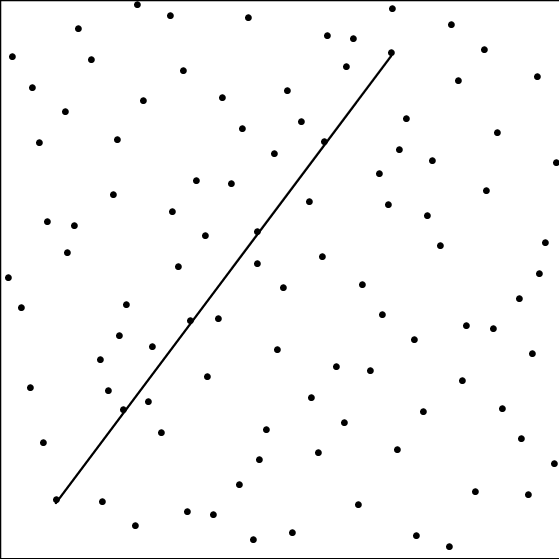
\includegraphics[width=6cm]{../png/hbequisp.png}}
\caption{Conceptual configuration.
A particle, indicated by the straight line, moves against a background thermal (`fluid')
species shown as dots.  In the refinement by De~Esch, interactions take place
at uniformly spaced intervals along the track, also indicated by dots\label{fig:hbequisp}}
\end{figure}

As illustrated in \Fig{hbequisp}, let $\tau (s)$ be the optical depth traversed by a 
article traveling a distance~$s$ through a medium 
with arbitrarily specified macroscopic cross-section~$\sigma(s)$: 
\begin{equation}\label{eq:optd}
\tau(s)= {\int_0}^s \sigma(s')ds'
\end{equation}
We assume only that $\sigma$ is finite and $\sigma(s)\ge 0$. Note that 
\begin{equation}\label{eq:doptd}
\frac{d \tau}{d s} = \sigma (s) 
\end{equation}
To explicitly allow for the case of no collision in a finite distance of travel, 
we define~$\mathrm{P}_{NC}$, the probability of no collisions, as 
\begin{equation}\label{eq:PNC}
\mathrm{P}_{NC} = \exp{(-\tau(\infty))}
\end{equation}
Then the probability density function (pdf) for a collision occurring after a particle has traveled a 
distance~$s$ through the medium is given by~\cite[\S\,7]{lewismiller}
\begin{equation}\label{eq:pdf}
\mathrm{p}(s)=\mathrm{P}_{NC} \delta(s-s_{\infty}) + \frac{d \tau}{d s} \exp{(-\tau(s))}
\end{equation}
where $\frac{d \tau}{d s}$ is the interaction probability per unit distance travelled,
$s_{\infty}$ is the distance to the boundary of the computational domain and
$\exp{(-\tau(s))}$ is the probability of traversing 
distance~$s$ without collision. \Eq{pdf} explicitly allows for cases where 
$\tau(\infty)$ is 
finite, hence there is a possibility of traveling an infinite distance without colliding.

Unbiased random sampling of the Monte Carlo path requires solving the
following for~$s$, distance along the path, 
namely
\begin{equation}\label{eq:xisamp}
\xi = {\int_0}^s \mathrm{p}(s')ds'
\end{equation}
where $\xi$ is sampled from a uniform random variable on~$[0,1)$. In the
spirit of
De~Esch, values of $\xi= j/N_{\xi}, j=1, \ldots N_{\xi}-1$ should be used,
and the charged particle weights (effectively the number of physical
particles each represents) be reduced by~$N_{\xi}$. Values of $N_{\xi} \approx
10-100$ are suggested.
 
In the first step of the sampling, discrete sampling is used to select a collision with probability $(1-\mathrm{P}_{NC})$
or an infinite flight with probability $\mathrm{P}_{NC}$. That is, 
if $\xi > \mathrm{P}_{NC}$, 
then there is a collision. The second step is to sample~$s$ from 
 from the pdf given by:
\begin{equation}\label{eq:partpdf}
g(s')=\frac{1}{G} \frac{d \tau}{d s'}\exp{(-\tau(s'))}
\end{equation}
where
\begin{equation}\label{eq:GPNC}
G= (1-\mathrm{P}_{NC})
\end{equation}
Using \Eq{partpdf}, note that 
\begin{equation}\label{eq:gconstr}
{\int_0}^s g(s')ds' = \frac{1}{G} {\int_0}^{\tau(s)} \exp{(-\tau)}d\tau
\end{equation}
Using \Eqs{xisamp}{partpdf}, we can sample $\tau_s=\tau(s)$ by solving 
\begin{equation}\label{eq:xiG}
\xi=\frac{1}{G} {\int_0}^{\tau_s} \exp{-\tau}d\tau
\end{equation}
This is equivalent to sampling from a truncated exponential pdf, which has 
the solution 
\begin{equation}\label{eq:xiGsoln}
\tau_s -\ln(1-G\xi)
\end{equation}
Pathlength $s$ then follows from \Eq{optd}, viz.
\begin{equation} \label{eq:sfromtau}
\tau_s ={\int_0}^s \sigma(s') ds'
\end{equation}
When $\sigma(s')$ has a simple functional form, \Eq{sfromtau} can often be solved analytically for~$s$. In many 
cases which arise in practice, the solution may involve a transcendental equation or other form 
not amenable to analytic solution. \Eq{sfromtau}, however, can be readily solved numerically for~$s$ 
using Newton iteration with $f= {\int_0}^s \sigma(s') ds' -s$,
starting with an initial estimate $s_0 = \tau_s/\sigma(0)$~\cite{Br03Dire}. 
Because $df/ds\le 0$, $f$ is monotone and there can be at most one root.
For cases where $\sigma(s')\ge 0$,
the Newton iteration is guaranteed to 
converge. However, if $\sigma(s')$ is zero or very small over a portion of the path, $df/ds$~may be~$0$,
leading to numerical difficulties and nonconvergence. This potential problem is 
remedied easily by combining Newton with a bisection search method, such that
bisection is used if $df/ds$ is very small or zero. Using this approach, Brown
and Martin 
found that only $1-5$~iterations are typically needed to converge~$s$ to within
part in $10^6$.
even for extreme variations in $\sigma(s')$. 

 
A final practical point concerns the relation of path length~$s$ to physical coordinates.
If the particle starts at~${\bf x}_0$ and travels in a direction
given by ${\bf v}_p$ parallel to unit vector~${\bf d}$ then the particle path is given by
\begin{equation}\label{eq:patheq}
{\bf x} = {\bf x}_0 + s {\bf d}
\end{equation}
so inverting
\begin{equation}\label{eq:zpatheq}
s = |{\bf x}-{\bf x}_0|/|{\bf d}|
\end{equation}
so it is helpful if ${\bf d}$ is a unit vector.

